\section{Concept}

\subsection{Neural Network}

For the neural network we base the architecture of our network on the well known \emph{LeNet} architecture from \cite{LeCun:1998aa} which is chosen due to its simplicity and ease to implement. Additionally the performance is improved by using modern, established techniques like batch normalization \cite{Ioffe:2015aa} and dropout \cite{Srivastava:2014aa} layers. 
The training of network is done using PyTorch \cite{Paszke:2019aa} on a regular PC and the trained network parameters are then used to create a hardware VHDL model of the network. An overview of the structure can be seen in Figure~\ref{fig:eggnet}. For verification all neural network operations are checked in separate programmed programs for correctness. See the Section~\ref{subsec:nntraining} for details how the network is implemented in Software.
An excellent overview in deep learning can be found in \cite{Schmidhuber:2015aa} and also in \cite{Goodfellow:2016aa}.
To train and test the network we chose the MNIST dataset \cite{LeCun:1998ab}. It consists of 50.000 training images and 10.000 test images of handwritten digits, where each has 28-by-28 pixel.

\begin{figure}[hbt]
	\centering
	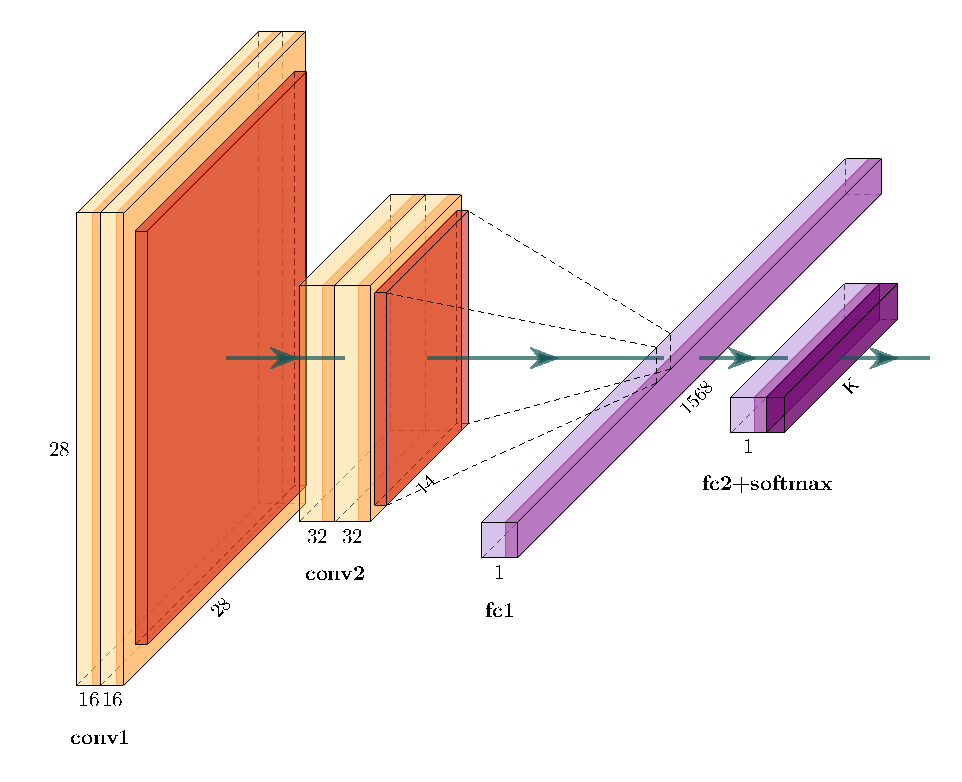
\includegraphics[width=0.6\textwidth]{img/eggnet}
	\caption{The Eggnet structure}
	\label{fig:eggnet}
\end{figure}


\subsection{Hardware Concept}
\begin{figure}[h]
	\centering
	\includesvg[width=0.8\textwidth]{img/inkscape/NN-concept.svg}
	\caption[Top-Level concept.]{Top-Level concept}
	\label{fig:hw-concept}
\end{figure}
\noindent
Figure \ref{fig:hw-concept} shows the Concept of implementing an FPGA-based hardware accelerator for handwritten digit recognition. A Zedboard is used as hardware platform, which includes a Zynq-7000 FPGA and provides various interfaces. It is also shown that the design can be remote controlled via a server which is running on the Zedboard. \\
A hardware accelerator for the neural network is implemented in the programmable logic part of the Zynq-7000. It is pre-trained using the remote PC, therefore only the inference of the neural network is implemented in hardware. \\
In order to train the network with the same bit resolution as implemented in the hardware, a software counterpart of the hardware is implemented in a PC using python. 
Based on the weights calculated by the python script a bitstream for the hardware is generated. This brings the benefit that for the convolutional layer constant multiplier can be used, since the weights of convolutional layer kernels are constant. For the dense layer it is not possible to implement the weights in a constant multiplier because in a dense layer each connection of a neuron requires a different weight, which would result in a huge amount of required constant multipliers. Therefore the weights for the dense layer have to be stored in a ROM inside the FPGA.   \\

